%%% Ne pas modifier jusqu'à la ligne 25
\documentclass[a4paper,12pt]{book}
\usepackage[utf8]{inputenc}
\usepackage[french]{babel}
%%\usepackage{CJK}
\usepackage{yhmath}
\usepackage{esint}
\usepackage[left=2cm,right=2cm,top=3cm,bottom=2cm, headheight=1.5cm,headsep=1.5cm]{geometry}
%%\usepackage{CJKutf8}
\usepackage{amsfonts}
\usepackage{mathrsfs}
\usepackage{amsmath,amsfonts,amssymb,dsfont}
\usepackage{graphicx}
\usepackage{array}
\usepackage{subfigure}
\usepackage{enumitem}		%\enumerate-resume
\usepackage{multirow}
\usepackage{multicol}
\usepackage{makecell}
\usepackage{pdflscape}
\usepackage{arydshln}
\usepackage[colorlinks=true,unicode={true},hyperindex=false, linkcolor=blue, urlcolor=blue]{hyperref}
\newcommand{\myref}[1]{\ref{#1} page \pageref{#1}}

\addto\captionsfrench{\def\tablename{Tableau}}  %légendes des tableaux
\renewcommand\thesection{\Roman{section}~-~} 
\renewcommand\thesubsection{\Roman{section}.\Alph{subsection}~-~} 
\renewcommand\thesubsubsection{\Roman{section}.\Alph{subsection}.\arabic{subsubsection}~-~} 

\newcommand{\conclusion}[1]{\newline \centerline{\fbox{#1}}}

\setcounter{secnumdepth}{3}
\parindent=0pt

\usepackage{fancyhdr}
\pagestyle{fancy}

\lhead{SJTU-ParisTech} 
%%%%%%%%%%%%%%%%%%%%%%%%%%%%%%%%%%
\chead{DM}
\rhead{Daniel 518261910024}

\begin{document}
\begin{landscape}
\renewcommand{\labelitemi}{$\blacktriangleright$}
\renewcommand{\labelitemii}{$\bullet$}


   
\section{synthèse comparative}
% \begin{figure}[h]
%     \begin{center}
%     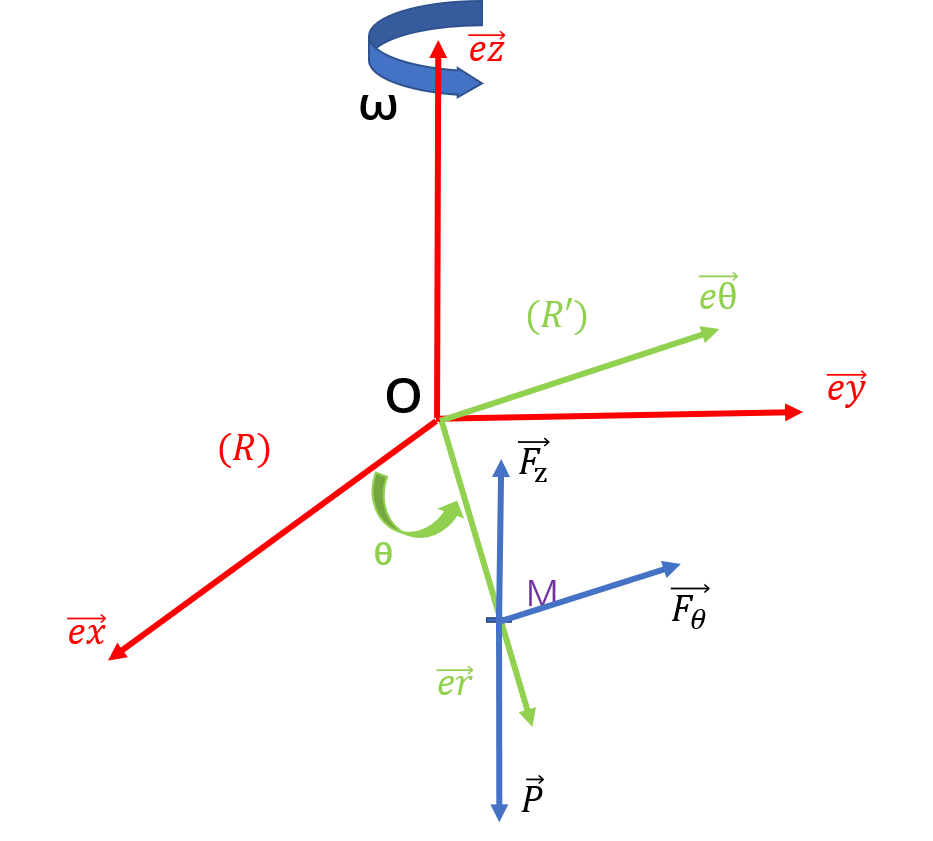
\includegraphics[scale=0.6]{meca41.png}
%     \end{center}
%     \caption{le système étudiée}
% \end{figure}
\begin{table}[h]
    \centering
    %\caption{The title of the table}

    %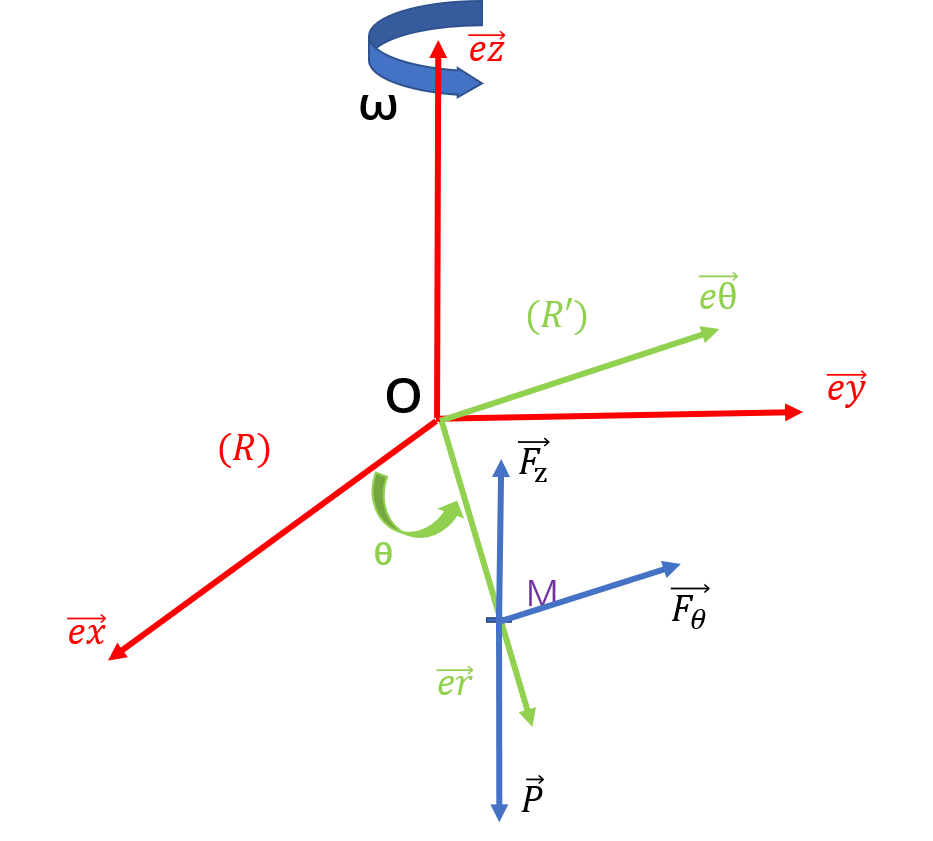
\includegraphics[scale=0.3]{meca41.png}
    \begin{tabular}{|m{4cm}<{\centering}|m{10cm}<{\centering}|m{10cm}<{\centering}|}
    \hline
    title & champs électrostatique & champs magnétostatique  \\
    \hline
    Sa définition à partir d’une loi de force  &la force électrostatique :
    $\vec{F}=q\vec{E}$  &la force de Lorentz magnétique $\vec{F}_{m \rightarrow M}=q_{M} \vec{v}_{M} \wedge \vec{B}(M)$\\ \hline


    Les formulations locales et intégrales des équations de Maxwell &
    La  formule locale sur la divergence du champ électrostatique$$ \operatorname{div} \vec{E}(M)=\frac{\rho(M)}{\varepsilon_{0}}$$

    La circulation le long d'un contour $(\mathscr{C})$ (circulation conservative de E)$$C=\oint_{(\mathscr{C})} \vec{E}(M) \cdot \overrightarrow{\mathrm{d} \ell}=0$$
    
    La  formule locale sur le rotationnel du champ électrostatique $$\overrightarrow{\operatorname{rot}} \vec{E}(M)=\overrightarrow{0}$$

    Le théorème de Gauss $$\varoiint_{P \in(S)} \vec{E}(P) \cdot \overrightarrow{\mathrm{d} S}_{P}=\frac{Q_{\text {int }}}{\varepsilon_{0}}$$
    
    & 
    La  formule locale sur la divergence du champ magnétostatique $$\operatorname{div} \vec{B}(M)=0$$

    Le flux à travers une surface fermée (flux conservatif de B) $$\Phi=\varoiint_{M \in(S)} \vec{B}(M) \cdot \overrightarrow{\mathrm{d} S}_{M}=0$$
    
    La  formule locale sur le rotationnel du champ magnétostatique $$\overrightarrow{\operatorname{rot}} \vec{B}(M)=\mu_{0} \vec{j}(M)$$

    
    Le théorème d'Ampère $$\oint_{P \in(\mathscr{C})} \vec{B}(P) \cdot \overrightarrow{\mathrm{d} \ell}_{P}=\mu_{0} I_{\text {int }}$$
    \\ \hline
    
    
    Ses propriétés de symétrie selon les propriétés de symétrie de la distribution source &
    Les propriétés de symétrie du champ électrostatique et de ses sources sont identiques & 
    Les propriétés de symétrie du champ magnétostatique et de ses sources sont opposées
    \\ \hline 
    
    
    
     \hline
    \end{tabular}
    \end{table}
\end{landscape}
    
\begin{landscape}
\begin{table}[h]
    \centering
    %\caption{The title of the table}

    %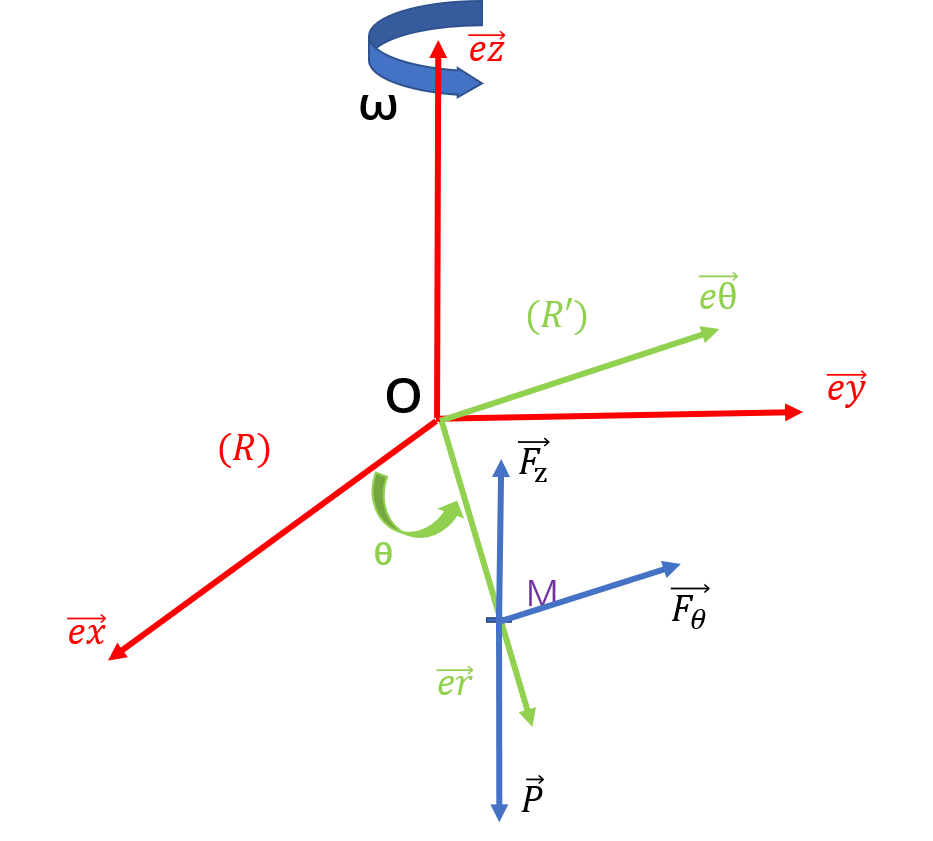
\includegraphics[scale=0.3]{meca41.png}
    \begin{tabular}{|m{4cm}<{\centering}|m{10cm}<{\centering}|m{10cm}<{\centering}|}
    \hline
     & champs électrostatique & champs magnétostatique  \\
    \hline
    Des informations sur sa topographie & Les lignes de champ électrostatique divergent à partir d'une charge positive et convergent
vers une charge négative. Les lignes de champ électrostatique divergent à partir d'une charge positive et convergent
vers une charge négative
&
Les lignes de champ magnétostatique divergent à partir d'un pôle magnétique nord (N) et convergent vers un pôle magnétique sud (S). 
Les lignes de champ magnétostatique se referment toujours sur elles-mêmes (ou à l'infini)\\ \hline 
    
    
    Son expression intégrale 
    & loi de Coulomb

        $$\vec{E}(M)=\frac{1}{4 \pi \varepsilon_{0}} \iiint_{P \in(V)} \frac{\rho(P) \mathrm{d} \tau_{P}}{P M^{2}} \vec{u}_{P M}$$

    & loi de Biot et Savart

    $$\vec{B}(M)=\oint_{P \in(\mathscr{C})} \frac{\mu_{0}}{4 \pi} \frac{I \overrightarrow{\mathrm{d} \ell_{P}} \wedge \vec{u}_{P M}}{P M^{2}}$$
    
    \\ \hline
    
    
    Ses propriétés de continuité selon la distribution 
    &
\begin{itemize}
    \item distribution volumique de charge: $\vec{E}(M)$ est défini et continu
    \item distribution surfacique de charge: $\vec{E}(M)$ subit une discontinuité à
    la traversée de la surface chargée
    \item distribution linéique de charge: $\vec{E}(M)$ n'est pas défini
\end{itemize}

    & 
    \begin{itemize}
        \item distribution volumique de charge: $\vec{B}(M)$ est défini et continu
        \item distribution surfacique de charge: $\vec{B}(M)$ subit une discontinuité à
        la traversée de la surface chargée
        \item distribution linéique de charge: $\vec{B}(M)$ n'est pas défini
    \end{itemize}
    
    
    \\ \hline
    
    
    Un exemple simple et rapide de calcul de champ 
    &
    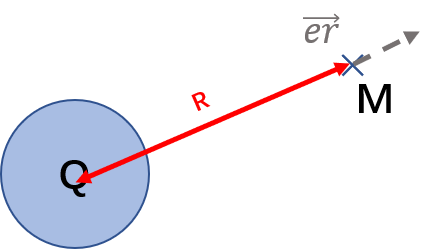
\includegraphics[scale=1]{elec31.png}

    %Une boule chargée de charge $Q$, en utilisant le théorème de Gauss

    $$\vec{E}(M)=\frac{3Q}{\epsilon_0 4\pi R^3}\vec{e}_r$$
    & 
    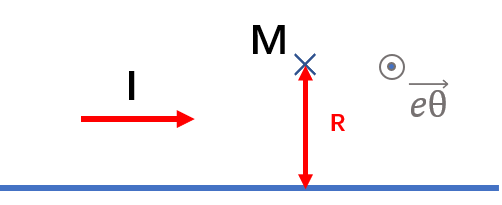
\includegraphics[scale=1]{elec32.png}

    $$\vec{B}(M)=\frac{\mu_0I}{2\pi R}\vec{e}_\theta$$

     \\
    
     \hline
    \end{tabular}
    \end{table}
\end{landscape}



\end{document}